\documentclass[11pt,a4paper]{article}
\usepackage[utf8]{inputenc}
\usepackage[spanish]{babel}
\usepackage{biblatex}
\usepackage{amssymb, amsmath, amsbsy}
\usepackage{graphicx}
\usepackage{makeidx}
\usepackage{color,xcolor}
\usepackage[left=2cm,right=2cm,top=2cm,bottom=2cm]{geometry}
\usepackage[linkcolor=black,colorlinks=true,urlcolor=blue]{hyperref}
\usepackage{xcolor}
\usepackage{fancyhdr}
\usepackage{float}
\usepackage{subfigure}
\renewcommand{\baselinestretch}{1.5}
\addbibresource{bib.bib}
\setlength{\parindent}{0em}
\bibliography{bib}

\begin{document}

\thispagestyle{empty}
\begin{center}

\includegraphics[width=10cm]{Graph/logo udesa.PNG}
\end{center}


	\begin{center}
	\LARGE
	Herramientas Computaciones para Investigación
\\			\vspace{1cm}
\hrule
	\vspace{0.5cm}
	\LARGE
 Avance de Proyecto Final
\\		
		\vspace{0.5cm}
		\hrule
				\vspace{1cm}
	\large

	\vspace{2.5cm}
	\large
		Alumnos:\\
	\large
	Elard Amaya, Francisco Guerrero
	
	
	\vspace{1.3cm}
	\normalsize	
	Profesora:\\

	\normalsize
	Amelia Gibbons
	
	\vspace{1.3cm}
	\today
	\end{center}

	
\clearpage
\section*{Nuevos gráficos}

Para el proyecto final, el artículo que hemos escogido es “On the Origins of Gender Roles: Women and the Plough”. La hipótesis principal de este artículo es que las sociedades que tradicionalmente practicaron la agricultura de arado, en lugar de la agricultura nómada (\textit{shifting cultivation}), tienen en la actualidad normas de género menos equitativas, lo cual debería reflejarse en una serie de indicadores relacionados al género como la participación de mujeres en el mercado laboral, la proporción de mujeres en actividad empresarial, etc.
\\
En principio, tomamos la base de datos pública del artículo y elaboramos dos mapas. El primer mapa (Figura 1) hace referencia a lo que los autores denominan el "cultivo con arado negativo", es decir, la capacidad de la tierra para sembrar cultivos que no se benefician de la agricultura por arado. Con este mapa, intentamos mostrar cuales fueron los paises menos propensos a practicar la agricultura de arado, dada las limitaciones que mostraban sus tierras. Lo que se esperaría, siguiendo la hipótesis del artículo, es que en los países donde la agricultura de arado era menos viable, en la actualidad, predominen normas de género más equitativas. 
\\
El segundo mapa (Figura 2) hace referencia a los países con mayor proporción de mujeres que cuentan con empresas propias, siguiendo la hipótesis del artículo, se esperaría que los países en los que se practicó la agricultura de arado, las proporciones de mujeres con empresas propias sea menor. 
\\
\begin{figure}[!h]
    \centering
    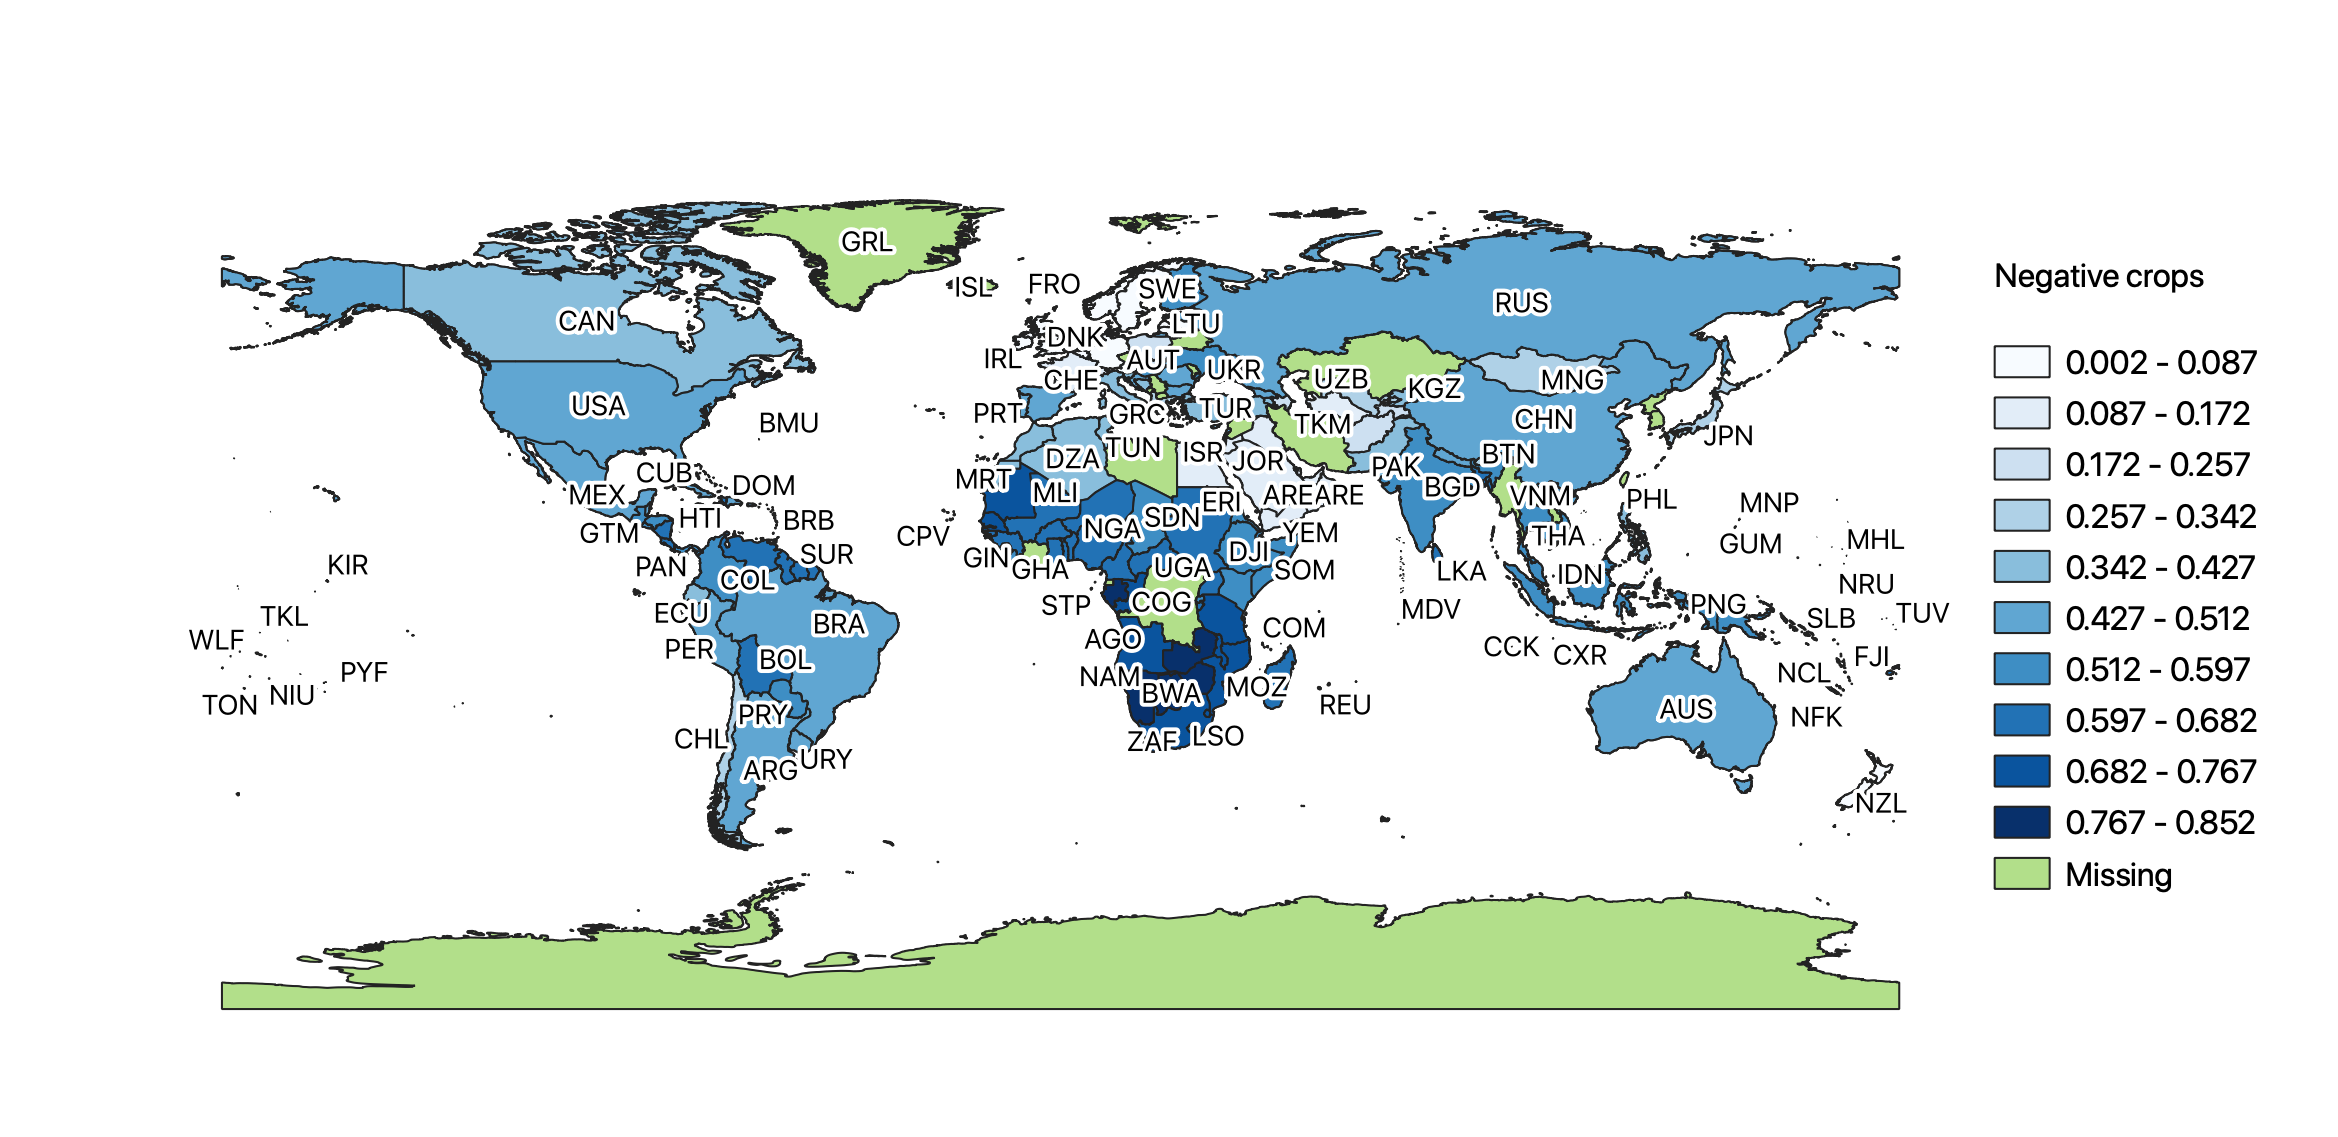
\includegraphics[width=15cm]{Graph/Graph 1.png}
   \caption{Tierras menos propensas para cultivos provenientes del arado}
    \label{fig:my_label}
\end{figure}

\begin{figure}[!h]
    \centering
    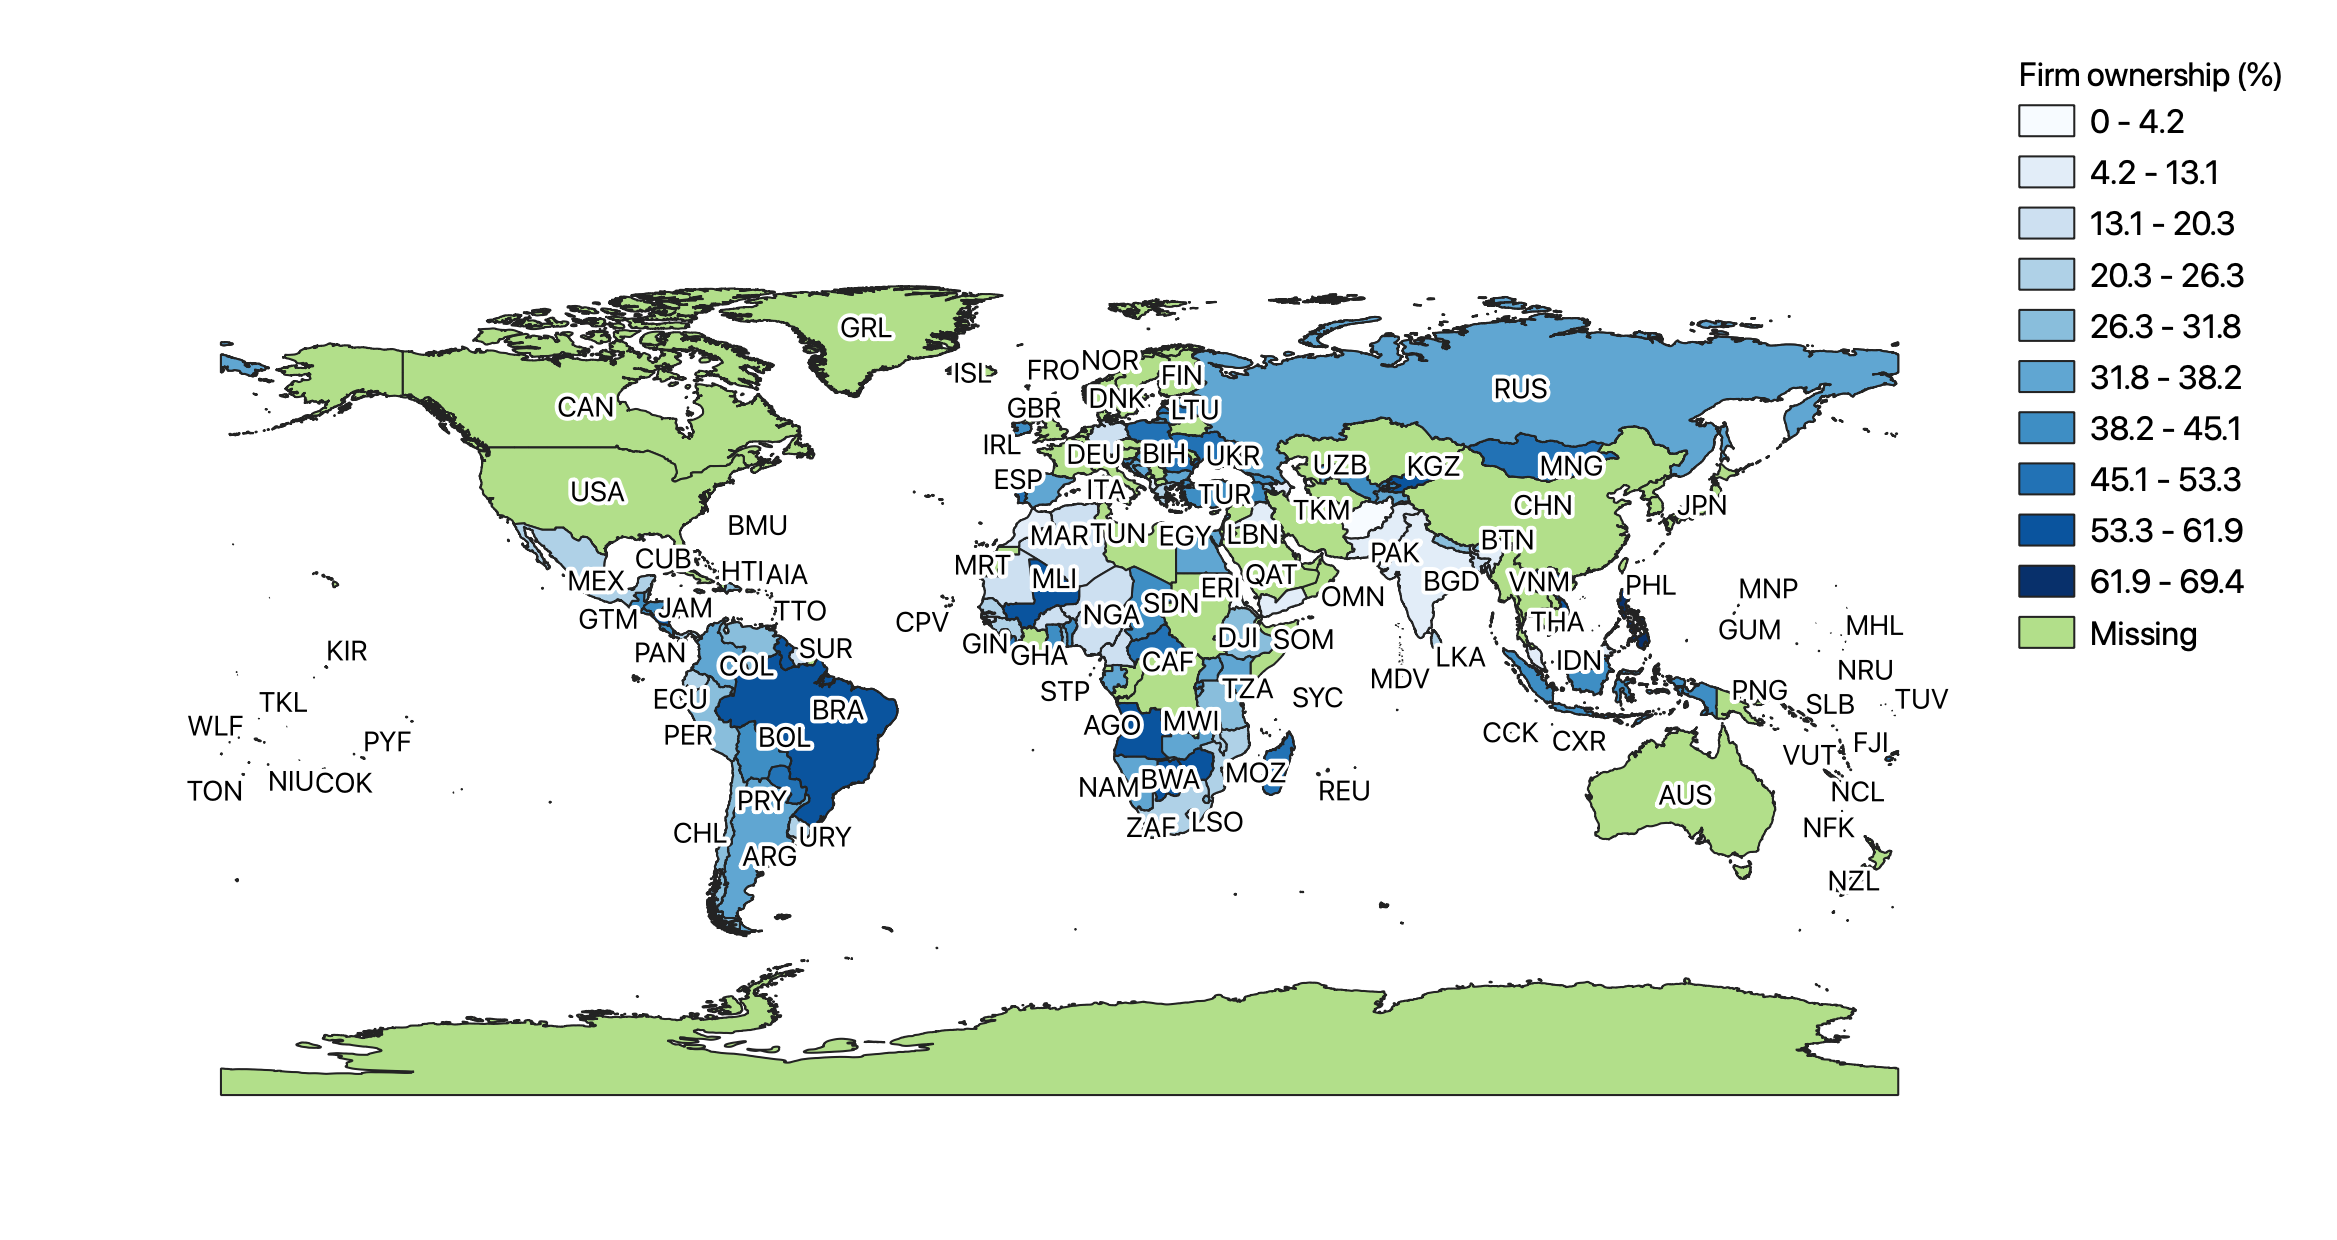
\includegraphics[width=15cm]{Graph/Graph 2.png}
   \caption{Mujeres con empresas propias (\%)}
    \label{fig:my_label}
\end{figure}

Como complemento, empleamos la información del World Bank Open Data, base de datos que cuenta con indicadores que nos permiten observar las desigualdades de género entre países. Podemos agregar esta información dado que contamos con el isocode de cada país. 
\\
La Figura 3 muestra la asociación entre la práctica de la agricultura por arado y la tasa de desempleo femenina en el 2000. Encontramos una asociación marginalmente positiva, es decir que los países donde se usó más el cultivo por arado tienen, en la actualidad, tasas de desempleo femenino más altas, idea que se alinea con la hipótesis general del artículo.

Finalmente, en la Figura 4, mostramos la asociación entre la práctica de la agricultura por arado y la proporción de escaños ocupados por mujeres en los parlamentos nacionales, para cada continente. Realizamos el análisis desagregado por continente, dado que en el artículo hacen mención a que la asociación global no tuvo significancia estadística. La información desagregada muestra patrones interesantes que se podrían alinear con la hipótesis general. Encontramos que en Africa a mayor práctica tradicional de cultivo por arado, menor es la proporción de mujeres que ocupan escaños en los parlamentos, mientras que en Norteamérica encontramos la asociación inversa. Por otro lado, no encontramos una relación en Asia ni en Sudamérica; y los casos de Europa y Ocenía deben revisarse con precaución dadas las pocas observaciones que cuentan con una agricultura completamente nómada o de arado.

\begin{figure}[!h]
    \centering
    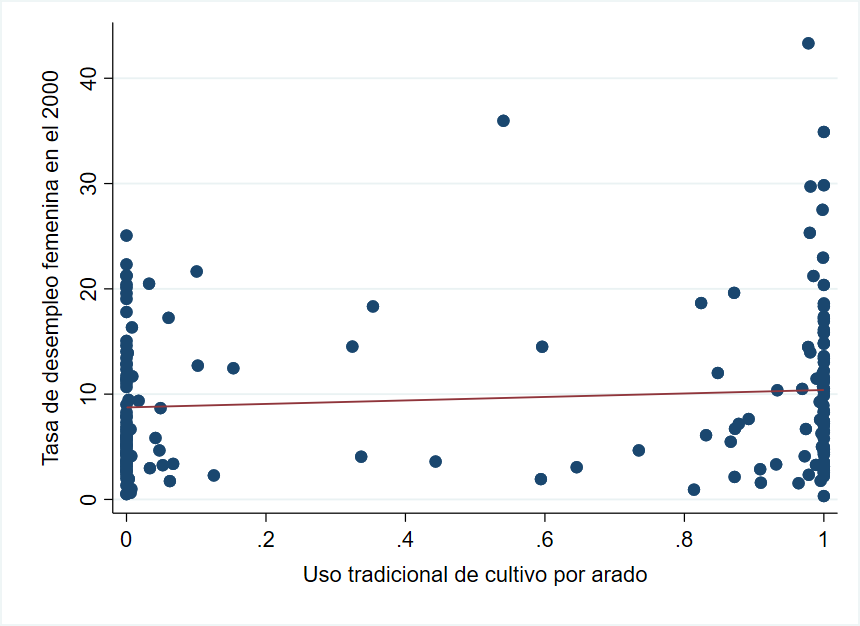
\includegraphics[width=15cm]{Graph/Graph 3.png}
   \caption{Relación entre cultivo por arado y tasa de desempleo femenina - 2000}
    \label{fig:my_label}
\end{figure}

\begin{figure}[!h]
    \centering
    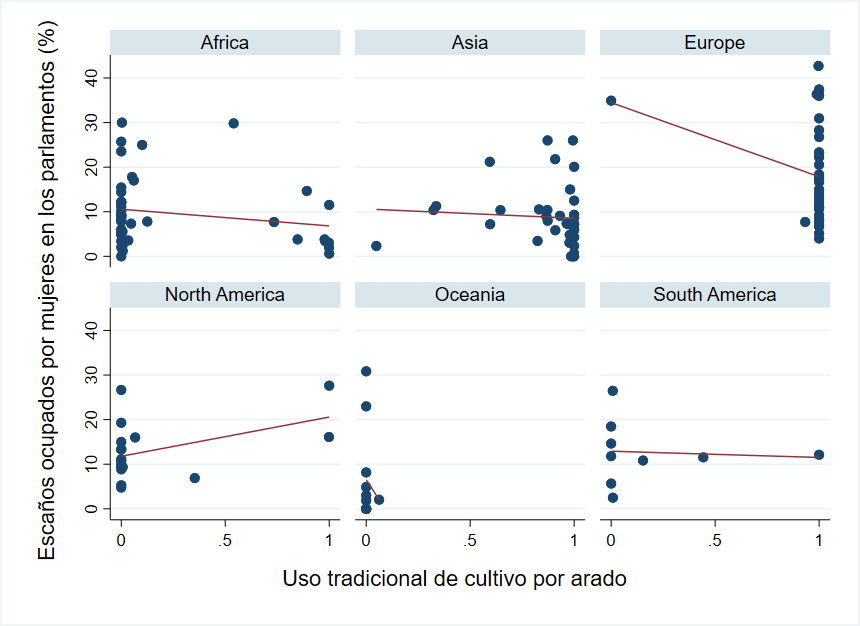
\includegraphics[width=15cm]{Graph/Graph 4.png}
   \caption{Relación entre cultivo por arado y participación de mujeres en política por continente - 2000}
    \label{fig:my_label}
\end{figure}

\end{document}
